\documentclass[12pt,article]{article}
\usepackage{fullpage}
\usepackage[top=2cm, bottom=4.5cm, left=2cm, right=2cm]{geometry}
\usepackage{amsmath,amsthm,amsfonts,amssymb,amscd}
\usepackage{lastpage}
\usepackage{enumerate}
\usepackage{fancyhdr}
\usepackage{mathrsfs}
\usepackage{xcolor}
\usepackage{graphicx}
\usepackage{listings}
\usepackage{hyperref}
\usepackage{mdframed}
\usepackage{changepage}   % for the adjustwidth environment
\usepackage{forest} 
\usepackage{tikz}   % For graph

\usepackage{float}  % To inforce inserting images at the right place

\usepackage{algorithm}
\usepackage{algpseudocode}

% For recursive formulation, adapted from https://tex.stackexchange.com/questions/580333/typing-sequences-recursively-in-overleaf
\usepackage{mathtools}
\makeatletter
\newcases{centercases}{\quad}
  {\hfil$\m@th\displaystyle{##}$\hfil}
  {$\m@th\displaystyle{##}$\hfil}{\lbrace}{.}
\makeatother

\newcommand{\Tau}{\mathrm{T}}


% For matrix
\def\horzbar{\text{magic}}

\hypersetup{%
  colorlinks=true,
  linkcolor=blue,
  linkbordercolor={0 0 1}
}

\setlength{\parindent}{0.0in}
\setlength{\parskip}{0.05in}

\newcommand\projnumber{1}
\newcommand\course{CS534}
\newcommand\OSUID{934370552}
\newcommand\Email{buivy@oregonstate.edu}
\newcommand\Name{Vy Bui}
\newcommand\tab[1][1cm]{\hspace*{#1}}

\pagestyle{fancyplain}
\headheight 35pt
\lhead{Practice Assignment \projnumber}
\rhead{Jan. 19, 2023}
\lfoot{}
\cfoot{}
\rfoot{\small\thepage}
\headsep 1.5em

\newenvironment{problem}[2][Problem]
    { \begin{mdframed}[backgroundcolor=gray!20] \textbf{#1 #2} \\}
    {  \end{mdframed}}
   

% Make Rightarrow with superscript
% \makeatletter
% \newcommand{\xRightarrow}[2][]{\ext@arrow 0359\Rightarrowfill@{#1}{#2}}
% \makeatother

\begin{document}

\begin{titlepage}
    \begin{center}
        \vspace*{4cm}

        \textbf{\Large CS515 - Algorithms \& Data Structures}

        \vspace{0.5cm}
 
        \textbf{\Large Practice Assignment 1}
 
        \vspace{1cm}

        Vy Bui - 934370552

        \vspace{2cm}

        Instructor: Professor Glencora Borradaile
        \vfill
             
        \vspace{0.8cm}
      
             
        The School of Electrical Engineering and Computer Science\\
        Oregon State University\\
             
    \end{center}
\end{titlepage}

%==============================================================================%
\begin{problem}{1} 
Suppose you are given an array A[1..n] of integers, which may be positive, negative, or zero. Describe a linear-time (i.e. O(n)-time) algorithm that finds the largest sum of elements in a contiguous, nonempty subarray A[i..j]. For example, given the array [-6, 12,-7, 0, 14,-7, 5] as input, your algorithm should return the integer 19 (the sum of [12,-7, 0, 14]).

For the sake of analysis, assume that comparing, adding, or multiplying any pair of numbers takes O(1) time.

\end{problem}

\textbf{Recursive Formulation}

First, let $MS(k)$ denote the function that find the nonempty contiguous subarray with the largest sum in $A[k:n]$. Second, let $MP(k)$ finds the contiguous subarray that starts from $k$ and has the largest sum. Note that $MPs$ can be empty. For example, let $A = [-3,-1,2,1]$, $MS(2) = 3, MP(2) = 2$, with the two last elements as MS and the last three elements as MP. However, $MS(1) = 3, MP(1) = 0$ with the two last elements as MS and the empty MP.

$MP$ and $MS$ can be defined recursively as follows:

\small{
    \[
        MP(k)=
        \begin{centercases}
            0                          & k > n \lor k \leq 0 \\
            max(0, A[k])               & k = n \\
            max(0, A[k] + MP(k+1))        & otherwise
        \end{centercases}
        \]
}

\small{
    \[
        MS(k)=
        \begin{centercases}
            0                  & k > n \lor k \leq 0 \\
            A[k]               & k = n \\
            max(A[k], A[k] + MP(k+1), MS(k+1))     & otherwise \\
        \end{centercases}
        \]
}

\normalsize{}

\textbf{Proof/Explanation}

\textit{Proof 1a}. For MP's recursive fomular, the first line prevents the algorithm to get out of the boundary of the subject array. In the base case on the second line, there is only one element in $A[k:k]$, so the result must be either empty or $A[k]$. For the inductive step, assume that $MP(k+1)$ returns the max prefix (contiguous subarray that starts from $k+1$ and has the largest sum) of $A[k]$, then $MP[k]$ must be $max(0, A[k] + MP(k+1))$. Because if there exists a larger prefix $A[k:j]$ so that $sum(A[k:j]) = A[k] + sum(A[k+1:j]) > A[k] + MP(k+1)$, then $sum(A[k+1:j] > MP(k+1))$, which contradicts the assumption that $MP(k+1)$ is the max prefix of $A[k+1:n]$. Proof completes.

\textit{Proof 1b}. For MS's recursive formula, the first line prevents the algorithm to get out of the boundary of the subject array. The second line is the base case in which we consider one element at the right end of the array. $A[k]$ is the only non-empty subarray in $A[k:k]$ so it must also be MS of $A[k:k]$. For the inductive step, assume that $MS(k+1)$ returns the max subarray of $A[k+1:n]$ and $MS(k+1)$ returns that max prefix, $MS(k)$ is guaranteed to be the maximum of the three case mentioned in the third line of the $MS(k)$ formula. Because if there exists a better solution, that is a contiguous subarray whose sum is greater than all of these cases, it will either contain $A[k]$ or not. In the first case when the subarray $S1$ does not contain $A[k]$, it must be within $A[k+1:n]$. $sum(S1) > MS(k+1)$ contradicts the assumption that $MS(k+1)$ is the max subarray of $A[k+1:n]$, hence there not exists such an subarray. In the second case where the subarray $S2$ contains $A[k]$, it can be decomposed to $sum(S2) = A[k] + sum(A[k+1:j])$. Again, $sum(S2) > A[k] + MP(k+1) \iff sum(A[k+i:j]) > MP(k+1)$ contradicts the assumption that $MP(k+1)$ is the max prefix, thus there not exists such an subarray. Proof completes!

\newpage
\textbf{Pseudocode}
Because $MS(k)$ only depends on $MS(k+1)$ and $MP(k)$ only depends on $MP(k+1)$, we can implement them iteratively in the same loop.

\begin{algorithm}
\caption{$(A[1:n])$}\label{alg:q1-LSA}
\begin{algorithmic}
    \State $ms \gets A[k]$\
    \State $mp \gets max(0, A[k])$\
    \State $k \gets n - 1$\;
    
    \While{$k \geq 1$}
        \State $mp \gets mp + A[k]$

        \State $max\_sum \gets max(A[k], ms, mp)$\

        \If{$mp == max\_sum$}
            \State $ms \gets mp$\
        \ElsIf{$A[k] == max\_sum$}
            \State $ms \gets A[k]$\
            \State $mp \gets A[k]$\
        \Else
            \State $mp \gets max(0, mp)$\
        \EndIf

        \State $k \gets k - 1$
    \EndWhile

    \Return $ms$
\end{algorithmic}
\end{algorithm}

\textbf{Runing Time and Space Analysis}
There are n iterations, each of which has constant number of operations, hence the algorithm has $O(n)$ time complexity. Furthermore, the algorithm uses $O(1)$ space.

%==============================================================================%
\newpage
\begin{problem}{2} 
String A is a supersequence of string B if string B can be obtained from string A by removing letters. For example, the strings BARNYARDSNACK, YUMMYBANANAS, and BWANWANWA are supersequences of the string BANANA. Give a dynamic program for finding the length of the shortest string that is a supersequence of two input strings A and B.
\end{problem}

We can create the shortest supersequence of A and B by modifying one of them to make it become a supersequence of the other with the least modifications. To keep the resulted sequence a supersequence of the starting string, only insertions are allowed. The proof will be given in the subsequent section. 

The problem now becomes finding the least number of insertions to turn one string to another. This resembles the Edit Distance problem mentioned in \cite{JeffE19} but simpler because it only allows insertions. Intuitively, starting with a longer string leads to less insertions, but both ways will result an optimal solution.

\textbf{Recursive Formulation}

Let $MI(i,j)$ denote the program that can return the minimum of insertions to transform $A[i:n]$ to a supersequence of $B[j:m]$. 

\normalsize{
    \[
        MI(i,j)=
        \begin{centercases}
            j   & i = 0 \\
            0   & j = 0 \\
            min(MI(i,j+1) + 1, MI(i+1,j+1)) & otherwise
        \end{centercases}
        \]
}

\textbf{Proof/Explanation}

Assume that we know the minimum number of insertions k needed to transform A to a supersequence S of B. S will be also a supersequence of A because we can always remove the inserted letters to transform it back to A. To prove that S is the shortest supersequence of A and B, proof by contradiction is used. Assume that there exists a shorter supersequence R of A and B. We can always transform A to R by only inserting some m letters into A. Because R is shorter than S, m is shorter than k, which contradicts with the assumption that k is the minimum number of insertions needed to transform A to a supersequence of B. Therefore, R does not exist and S is the shortest supersequence of A and B.

\textbf{Pseudocode}

\textbf{Runing Time Analysis}

%==============================================================================%
\newpage
\begin{problem}{3} 
Find the length (number of edges) of the longest path in a binary tree.
\end{problem}

\textbf{Observation 1:} A binary tree T includes two subtrees L and R, and the root node. The longest path of T, LP(T) can be a path within L, a path within R (2), or a combination of the longest path from the root node to some node in L and the longest path from the root node to some node in R (3). The longest path from some node in L to the root node is the depth of L + 1, and the same applies to R.

\textbf{Observation 2:} The depth of tree T, D(T), is the largest of the depth of the left subtree and the depth of the right subtree.

\textbf{Recursive Formulation}
\normalsize{
\[
    D(T)=
    \begin{centercases}
        -1   & T = \emptyset \\
        0    & T.L = \emptyset \land T.R = \emptyset \\
        1 + max(D(L), D(R)) & otherwise
    \end{centercases}
\]
}

\normalsize{
\[
    LP(T)=
    \begin{centercases}
        -1   & T = \emptyset \\
        0    & T.L = \emptyset \land T.R = \emptyset \\
        max(LP(L), LP(R), D(L) + D(R) + 2) & otherwise
    \end{centercases}
\]
}

\textbf{Proof/Explanation}

We will prove that there not exist a path in T that is longer than LP(L), LP(R), and D(L) + D(R) + 2, using proof by contradiction. Assume that there exists a longer path $(x,y)$ with $x,y \in L \cup R \cup r$ where $r$ is the root node. If $x,y \in L$, then it contradicts with the assumption that LP(L) is the longest path in L, which shows that such path does not exist. The same argument can be applied to path within the right tree. Lastly, if $x \in L$ and $y \in R$ then it has to go through r. We can break the path into two pieces, $(x,r)$ and $(r,y)$ so that $|(x,y)| = |(x,r)| + |(r,y)|$, which can not be greater than D(L) + D(R). Thus, such a path does not exist.

\newpage
\textbf{Pseudocode}
For this problem, a recursive implementation seems to be more efficient, readable, and easier to implement compared to an iterative implementation.

\begin{algorithm}
\caption{$D(T)$}\label{alg:q3-D}
\begin{algorithmic}
    \If{$T == \emptyset$}
        \Return -1
    \EndIf

    \If{$T.L == \emptyset \land T.R == \emptyset$}
        \Return 0
    \EndIf

    \Return $1 + max(D(T.L), D(T.R))$
\end{algorithmic}
\end{algorithm}

\begin{algorithm}
\caption{$LP(T)$}\label{alg:q3-LP}
\begin{algorithmic}
    \If{$T == \emptyset$}
        \Return -1
    \EndIf

    \If{$T.L == \emptyset \land T.R == \emptyset$}
        \Return 0
    \EndIf

    \Return $max(LP(T.L), LP(T.R), D(T.L) + D(T.R) + 2)$
\end{algorithmic}
\end{algorithm}

\textbf{Runing Time Analysis}

The iterative implementation needs to compute LP from the bottom up, that is from the leaves up to the root. The problem is we do not know the leaves in advance so it needs to traverse the trees one more time to find the leaves. For memory, it needs O(n) of memory to keep the results in the worst case that the tree is a full binary tree, which has (n + 1) / 2 leaves. On the other hand, a recursive algorithm only needs to traverse through the tree once because a node depends on exactly its two children nodes. Therefore, it takes O(n) time and O(n) space of stack to store the recursive calls.

%==============================================================================%
\newpage
\begin{problem}{4} 
Suppose you are given an n x n bitmap, represented by a 2-dimensional array M[1..n, 1..n] of 0s and 1s. A solid block in M is a subarray of the form M[i..i', j..j'] containing only 1s. Describe an algorithm to find the area of the maximum solid block in M in $O(n^3)$ time. If you can do that, try to design a faster algorithm that runs in $O(n^2)$ time.
\end{problem}

\underline{Observation 1}: Let us call the maximum solid block of $M[1:n,1:n]$ as $MSB[i:i',j:j']$. Observe that $MSB[i:i',j:j']$ is also the maximum solid block of the "sub-right-bottom-matrix" $M[i:n,j:n]$. A maximum solid block in $M$ is guaranteed to be the maximum solid block of the some of the sub-right-bottom-matrices. The maximum of the MSB of these sub-matrices is the final solution to the problem.

\textbf{Recursive Formulation}
Let us call the first dimension of the matrix as height, and the second dimension as width. Let $R(i,j)$ denotes the rectangle $M[i:n,j:n]$. Let $W[i,j]$ be the width of the widest block in $R(i,j)$ that contains $M[i,j]$ and has height of one, as shown by the green block in Figure \ref{fig:q4-notations}. Let $H[i,j]$ be the height of the tallest solid block in $R(i,j)$ that contains $M[i,j]$ and has width of one, as shown by the blue block in Figure \ref{fig:q4-notations}. Let $L[i,j] = (h,w)$ be the height and width of the largest solid block in $R(i,j)$ that contains $M[i,j]$, as shown by the red block in Figure \ref{fig:q4-notations}.

\begin{figure}[H]
    \centering
    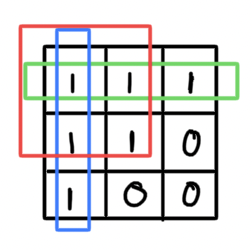
\includegraphics[scale=0.7]{notation.png} \par
    \caption{Suboptimal structure. The solution to the black rectangle depends on the solutions to the green, blue, and red rectangles}
    \label{fig:q4-notations}
\end{figure}

\begin{figure}[H]
    \centering
    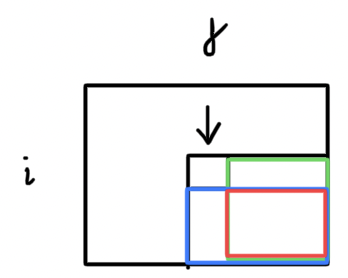
\includegraphics[scale=0.7]{recursion.png} \par
    \caption{Suboptimal structure. The solution to the black rectangle depends on the solutions to the green, blue, and red rectangles}
    \label{fig:q4-suboptimal-structure}
\end{figure}

The recursive formulations of those functions/tables can be defined as follows


\small{
\[
    W[i,j]=
    \begin{centercases}
        0               & M[i,j] = 0 \\
        \begin{centercases}
            0               & j = n \\
            1 + W[i,j+1]    & otherwise \\
        \end{centercases} & otherwise \\
    \end{centercases}
\]
}

\small{
\[
    H[i,j]=
    \begin{centercases}
        0               & M[i,j] = 0\\
        \begin{centercases}
            0               & i = n \\
            1 + H[i+1,j]    & otherwise \\
        \end{centercases} & otherwise \\
    \end{centercases}
\]
}

\small{
\[
    L[i,j]=
    \begin{centercases}
        (0,0)               & i,j < 1 \lor i,j > n \\
        (0,0)               & H[i,j] = 0\\
        \begin{centercases}
            (H[i,j],1)    & \\
            (1,W[i,j])    & \\
            (min(H[i,j], L[i+1,j+1][0] + 1), min(W(i,j), L[i+1,j+1][1] + 1)) & \\
        \end{centercases} & otherwise\\
    \end{centercases}
\]
}

\normalsize{}

In the otherwise case (line 3,4,5) of the formula $L[i,j]$, the program find the largest solid block between $H[i,j]$, $W[i,j]$, and $min(H[i,j], L[i+1,j+1][0] + 1) \times min(W(i,j), L[i+1,j+1][1] + 1)$.

\textbf{Proof/Explanation}

\textit{Proof 4a. }

\underline{Base case}: for rectangles whose top-left corner is on the right edge of $M$, the widest solid blocks obviously have width of one, if they exists.

\underline{Inductive Hypothesis}: assume that $W[i,j+1]$ is the width of the widest block in $R(i,j)$ that contains $M[i,j]$ and has height of one.

\underline{Inductive Step}: assume that there exists some $k$ that $W[i,j] = |M[i,j:k]| > W[i,j+1] + 1$. Removing $M[i,j]$ from $M[i,j:k]$ results in $M[i,j+1:k]$, which contains $M[i,j]$ and longer than $W[i,j+1]$. This contradicts the assumption that $W[i,j+1]$ is the width of the widest block in $R(i,j)$ that contains $M[i,j]$ and has height of one, which shows that $W[i,j] = W[i,j+1] + 1$ is true.

The same reasoning can be used for $H[i,j]$ recursive formulation.

\textit{Proof 4b. } 

\underline{Base case}: for rectangles whose top-left corner is on the right edge of $M$, the largest solid blocks obviously have size equal its $H$. Similarly, for rectangles whose top-left corner is on the bottom edge of $M$, the largest solid blocks obviously have size equal its $W$.

\underline{Inductive Hypothesis}: assume that $L[i+1,j+1]$ are the height and width of the largest solid block in $R(i,j)$ that contains $M[i,j]$.

\underline{Inductive Step}: by looking at Figure \ref{fig:q4-suboptimal-structure}, it is obvious that $L[i,j]$ must be one of the three mentioned in the formula. First, the block has to be within the bound of $W[i,j]$ and $H[i,j]$, the otherwise contradicts the assumption of $W[i,j]$ or $H[i,j]$. Second, the right-bottom corner of the block has to be within $L[i+1,j+1]$, otherwise, $L[i+1,j+1]$ is not the largest solid block of $R(i,j)$. Proof completes!

\textbf{Pseudocode}
\begin{algorithm}
\caption{$M[1:n,1:n]$}\label{alg:q4-L}
\begin{algorithmic}
    \If{$M == \emptyset$}
        \Return 0
    \EndIf

    \State $maxArea \gets 0$, $W \gets []$, $H \gets []$, $L \gets []$, $i \gets n$, $j \gets n$

    \While{$i \geq 1$}
        \While{$j \geq 1$}
            \If{$M[i,j] == 0$}
                \State $W[i,j] \gets 0$, $H[i,j] \gets 0$, $L[i,j] \gets (0,0)$\
            \ElsIf{$j == n \land i == n$}
                \State $W[i,j] \gets 1$, $H[i,j] \gets 1$, $L[i,j] \gets (1,1)$\
            \ElsIf{$j == n$}
                \State $W[i,j] \gets 1$, $H[i,j] \gets H[i+1,j] + 1$, $L[i,j] \gets H[i,j]$\
            \ElsIf{$i == n$}
                \State $W[i,j] \gets W[i,j+1]$, $H[i,j] \gets 1$, $L[i,j] \gets W[i,j]$\
            \Else
                \State $W[i,j] \gets W[i,j+1] + 1$\
                \State $H[i,j] \gets H[i+1,j] + 1$\
                \State $lh \gets min(H[i,j], L[i+1,j+1][0] + 1)$\
                \State $lw \gets min(W(i,j), L[i+1,j+1][1] + 1)$\
                \State $lArea \gets lh * lw$\
                \State $largestBlock \gets max(H[i,j], W[i,j], crossArea)$\

                \If{$lArea == largestBlock$}
                    \State $L[i,j] \gets (lh,lw)$\
                \ElsIf{$W[i,j] == largestBlock$}
                    \State $L[i,j] \gets (1,W[i,j])$\
                \Else
                    \State $L[i,j] \gets (H[i,j],1)$\
                \EndIf

                \State $maxArea \gets max(maxArea, largestBlock)$\
            \EndIf

            \State $j \gets j - 1$
        \EndWhile

        \State $i \gets i - 1$
    \EndWhile

    \Return $maxArea$
\end{algorithmic}
\end{algorithm}

\newpage
\textbf{Runing Time Analysis}

For time complexity, because the code in the inner loop takes constant time, the algorithm takes $O(n^2)$ in total. For space complexity, Algorithm \ref{alg:q4-L} consumes $O(n^2)$ space to store the $W,H,L$ tables for the entire $M$. However, notice that $L(i,j)$ only depends on the row below and the right cell. Therefore, we only need to keep track of $W,H,L$ tables of $M[i+1,1:n]$ and $M[i,j+1]$, thus reduce the space complexity to $O(n)$.

\newpage
\bibliographystyle{alpha}
\bibliography{mybib}
\end{document}
